\documentclass{article}\usepackage[]{graphicx}\usepackage[]{color}
%% maxwidth is the original width if it is less than linewidth
%% otherwise use linewidth (to make sure the graphics do not exceed the margin)
\makeatletter
\def\maxwidth{ %
  \ifdim\Gin@nat@width>\linewidth
    \linewidth
  \else
    \Gin@nat@width
  \fi
}
\makeatother

\definecolor{fgcolor}{rgb}{0.345, 0.345, 0.345}
\newcommand{\hlnum}[1]{\textcolor[rgb]{0.686,0.059,0.569}{#1}}%
\newcommand{\hlstr}[1]{\textcolor[rgb]{0.192,0.494,0.8}{#1}}%
\newcommand{\hlcom}[1]{\textcolor[rgb]{0.678,0.584,0.686}{\textit{#1}}}%
\newcommand{\hlopt}[1]{\textcolor[rgb]{0,0,0}{#1}}%
\newcommand{\hlstd}[1]{\textcolor[rgb]{0.345,0.345,0.345}{#1}}%
\newcommand{\hlkwa}[1]{\textcolor[rgb]{0.161,0.373,0.58}{\textbf{#1}}}%
\newcommand{\hlkwb}[1]{\textcolor[rgb]{0.69,0.353,0.396}{#1}}%
\newcommand{\hlkwc}[1]{\textcolor[rgb]{0.333,0.667,0.333}{#1}}%
\newcommand{\hlkwd}[1]{\textcolor[rgb]{0.737,0.353,0.396}{\textbf{#1}}}%

\usepackage{framed}
\makeatletter
\newenvironment{kframe}{%
 \def\at@end@of@kframe{}%
 \ifinner\ifhmode%
  \def\at@end@of@kframe{\end{minipage}}%
  \begin{minipage}{\columnwidth}%
 \fi\fi%
 \def\FrameCommand##1{\hskip\@totalleftmargin \hskip-\fboxsep
 \colorbox{shadecolor}{##1}\hskip-\fboxsep
     % There is no \\@totalrightmargin, so:
     \hskip-\linewidth \hskip-\@totalleftmargin \hskip\columnwidth}%
 \MakeFramed {\advance\hsize-\width
   \@totalleftmargin\z@ \linewidth\hsize
   \@setminipage}}%
 {\par\unskip\endMakeFramed%
 \at@end@of@kframe}
\makeatother

\definecolor{shadecolor}{rgb}{.97, .97, .97}
\definecolor{messagecolor}{rgb}{0, 0, 0}
\definecolor{warningcolor}{rgb}{1, 0, 1}
\definecolor{errorcolor}{rgb}{1, 0, 0}
\newenvironment{knitrout}{}{} % an empty environment to be redefined in TeX

\usepackage{alltt}
\IfFileExists{upquote.sty}{\usepackage{upquote}}{}
\begin{document}

\begin{knitrout}
\definecolor{shadecolor}{rgb}{0.969, 0.969, 0.969}\color{fgcolor}\begin{kframe}
\begin{alltt}
\hlcom{#GUIA 24 }

\hlcom{#AN�LISIS DE VARIANZA}

\hlcom{#Ejemplo 1}

\hlstd{notas} \hlkwb{<-} \hlkwd{c}\hlstd{(}\hlnum{20}\hlstd{,}\hlnum{18}\hlstd{,}\hlnum{18}\hlstd{,}\hlnum{23}\hlstd{,}\hlnum{22}\hlstd{,}\hlnum{17}\hlstd{,}\hlnum{15}\hlstd{,}\hlnum{13}\hlstd{,}\hlnum{21}\hlstd{,}\hlnum{15}\hlstd{,}\hlnum{20}\hlstd{,}\hlnum{13}\hlstd{,}\hlnum{12}\hlstd{,}\hlnum{16}\hlstd{,}\hlnum{17}\hlstd{,}\hlnum{21}\hlstd{,}\hlnum{15}\hlstd{,}
           \hlnum{13}\hlstd{,}\hlnum{12}\hlstd{,}\hlnum{15}\hlstd{,}\hlnum{18}\hlstd{,}\hlnum{20}\hlstd{,}\hlnum{18}\hlstd{,}\hlnum{17}\hlstd{,}\hlnum{10}\hlstd{,}\hlnum{24}\hlstd{,}\hlnum{16}\hlstd{)}
\hlstd{programas} \hlkwb{<-} \hlkwd{gl}\hlstd{(}\hlkwc{n}\hlstd{=}\hlnum{3}\hlstd{,} \hlkwc{k}\hlstd{=}\hlnum{9}\hlstd{,} \hlkwc{labels}\hlstd{=}\hlkwd{c}\hlstd{(}\hlstr{"P1"}\hlstd{,} \hlstr{"P2"}\hlstd{,} \hlstr{"P3"}\hlstd{))}
\hlstd{datos} \hlkwb{<-} \hlkwd{data.frame}\hlstd{(}\hlkwc{notas} \hlstd{= notas,} \hlkwc{programas} \hlstd{= programas);datos}
\end{alltt}
\begin{verbatim}
##    notas programas
## 1     20        P1
## 2     18        P1
## 3     18        P1
## 4     23        P1
## 5     22        P1
## 6     17        P1
## 7     15        P1
## 8     13        P1
## 9     21        P1
## 10    15        P2
## 11    20        P2
## 12    13        P2
## 13    12        P2
## 14    16        P2
## 15    17        P2
## 16    21        P2
## 17    15        P2
## 18    13        P2
## 19    12        P3
## 20    15        P3
## 21    18        P3
## 22    20        P3
## 23    18        P3
## 24    17        P3
## 25    10        P3
## 26    24        P3
## 27    16        P3
\end{verbatim}
\begin{alltt}
\hlstd{mod1} \hlkwb{<-} \hlkwd{aov}\hlstd{(notas} \hlopt{~} \hlstd{programas,} \hlkwc{data} \hlstd{= datos)}
\hlkwd{plot}\hlstd{(mod1)}
\end{alltt}
\end{kframe}
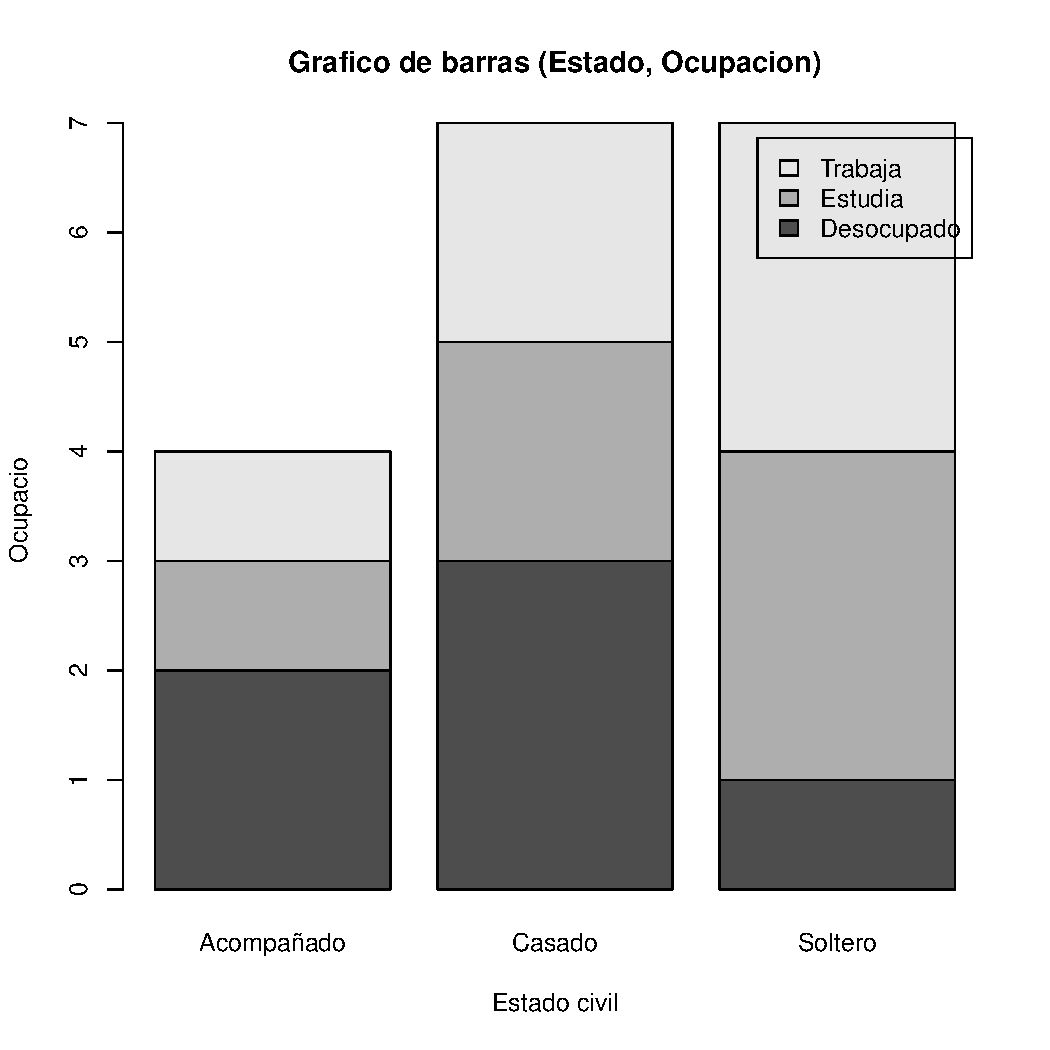
\includegraphics[width=\maxwidth]{figure/unnamed-chunk-1-1} 

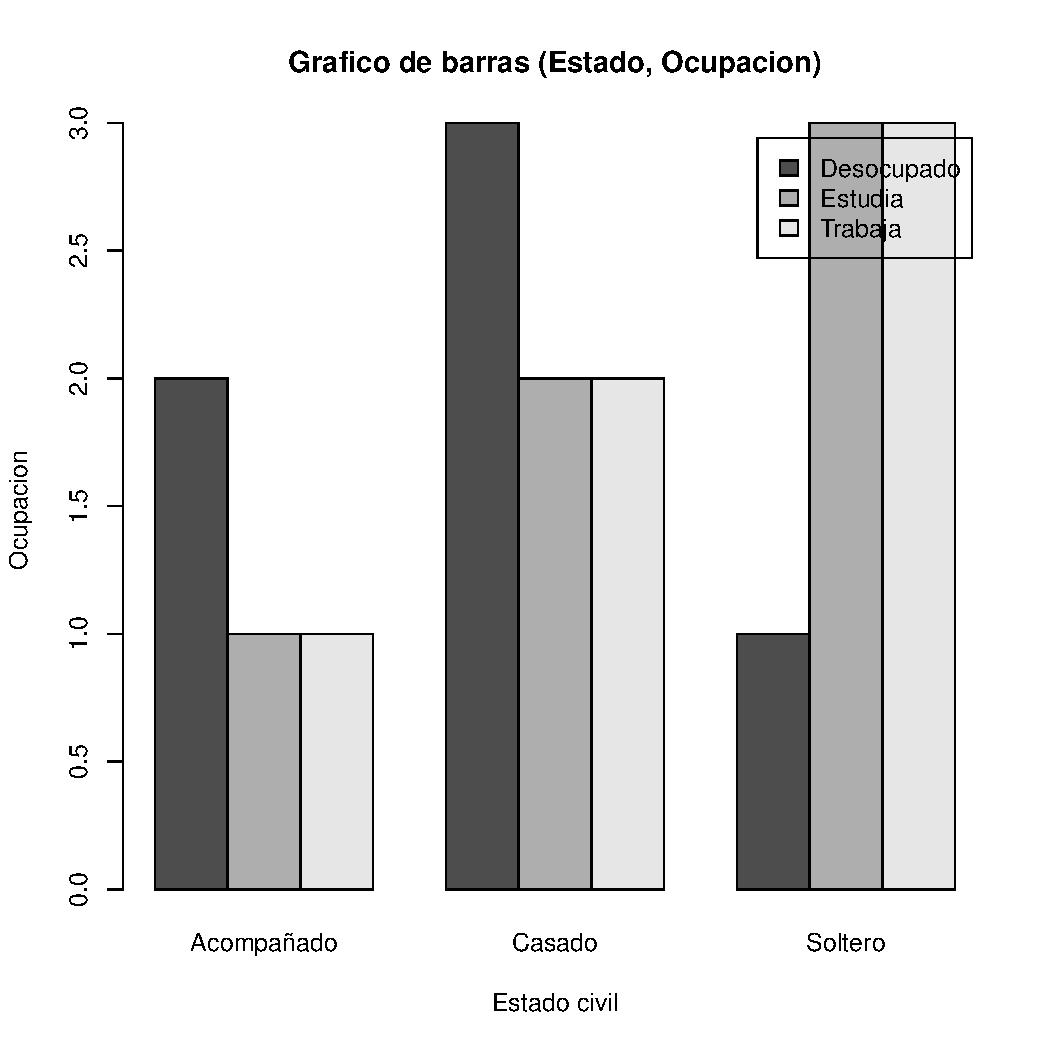
\includegraphics[width=\maxwidth]{figure/unnamed-chunk-1-2} 

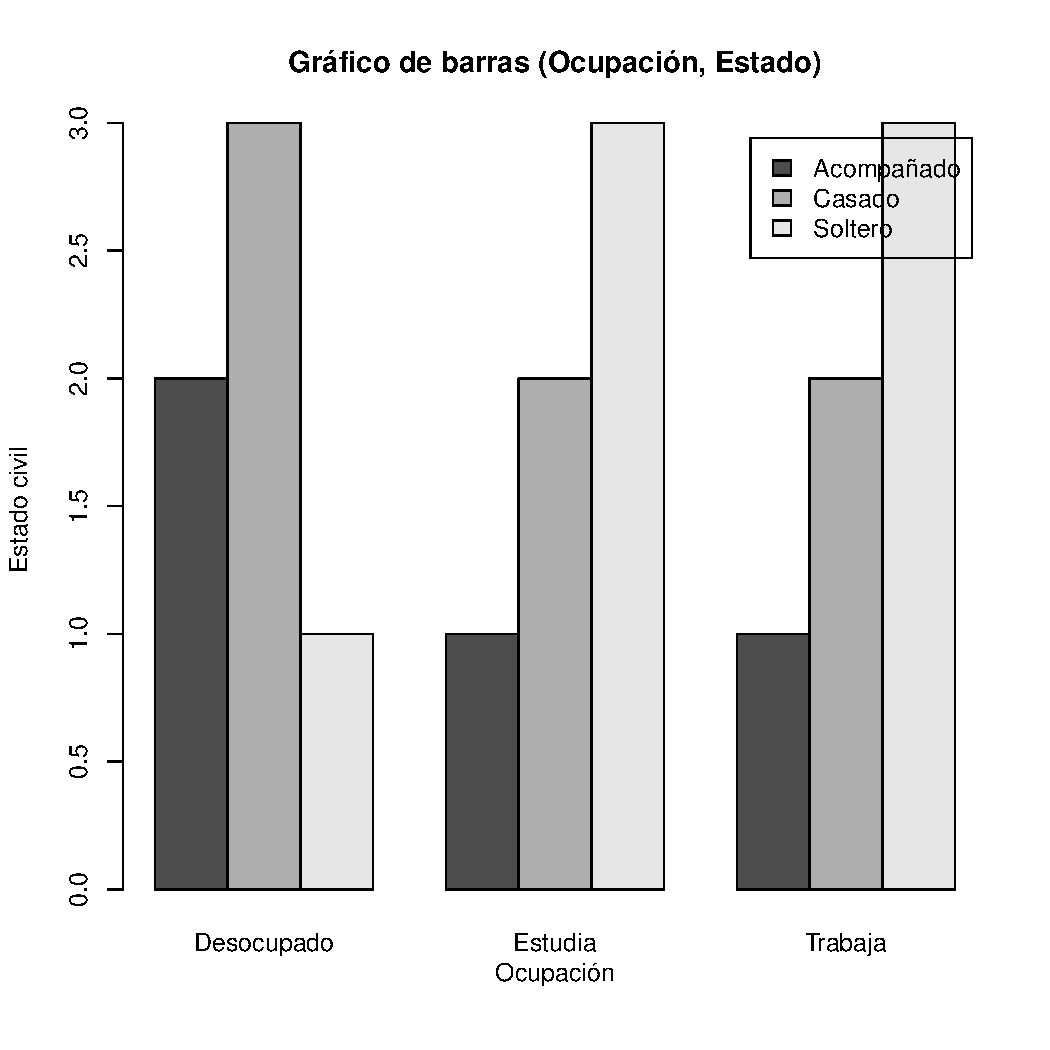
\includegraphics[width=\maxwidth]{figure/unnamed-chunk-1-3} 

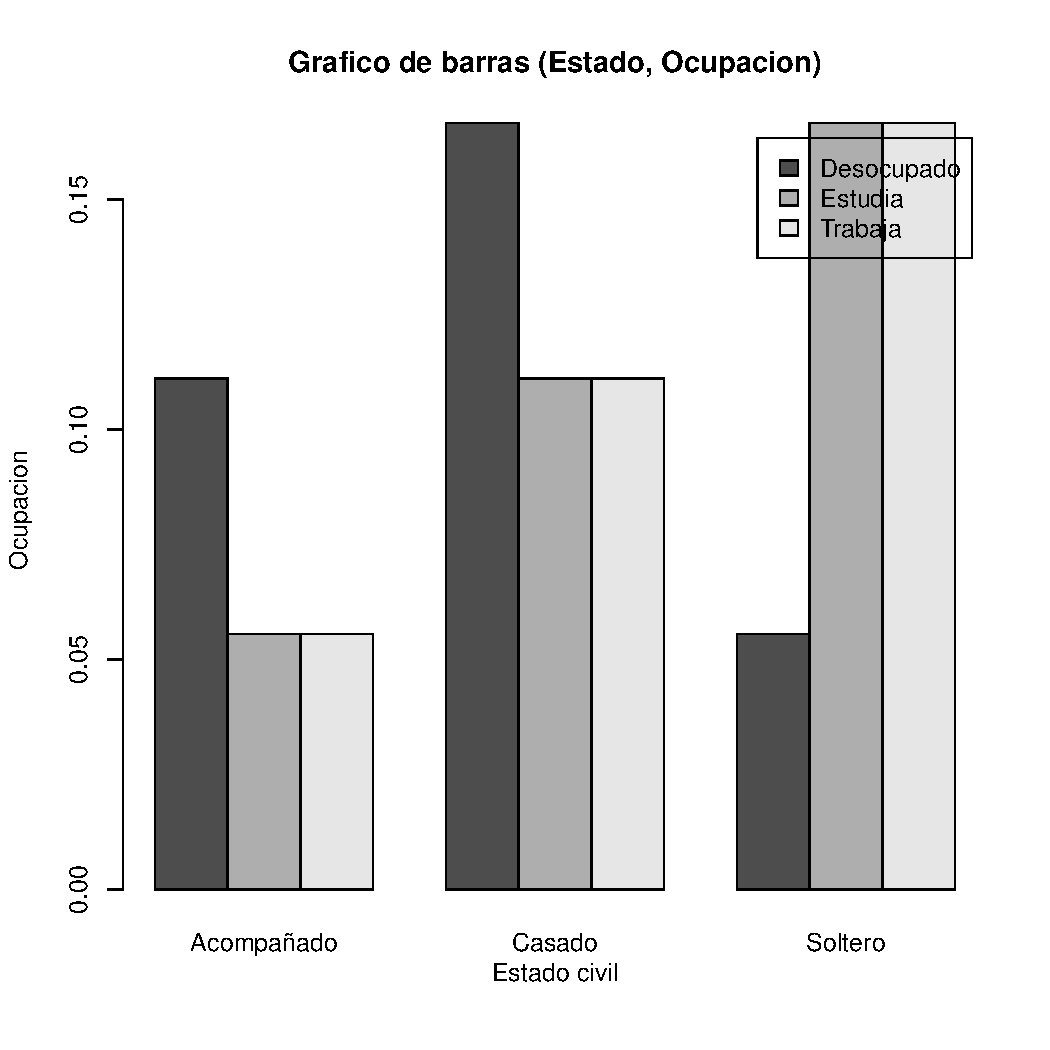
\includegraphics[width=\maxwidth]{figure/unnamed-chunk-1-4} 
\begin{kframe}\begin{alltt}
\hlcom{#Ejemplo 2}
\hlcom{#(No esta la base de datos)}
\end{alltt}
\end{kframe}
\end{knitrout}



\end{document}
